\section{Dataset Development}


% \section{Setup}

% The test object is a Festo Didactic System, which consists of a tool table with a rail field that can be freely equipped with various pneumatic elements. By means of this modular system, a simple pneumatic circuit is to be implemented. The use-cases of a a leaking connection point and worn tubing is simulated. Here the leakage noises are generated by a combination of a choke vent (CV1) with another choke vent (CV2) or folded tubing. CV1 regulates the airflow by turning a knurled screw that generates variable flow resistance. 

% \subsection{Microphone setup}

% For optimum recording of the leakage noise, microphones with an omnidirectional characteristic and sufficiently linear frequency response in the range 1 - 20 kHz is used (Earthworks M30). Eight microphones are paired to four fixed positions.  Two microphone positions with 6 cm and 60 cm are held by markings. The microphone is directed laterally towards the valve in order to obtain as much as possible of the sound field discussed in chapter 2.5 of the escaping free jet.

%  \begin{minipage}{\textwidth}
%   \begin{minipage}[b]{0.49\textwidth}
%     \centering
%     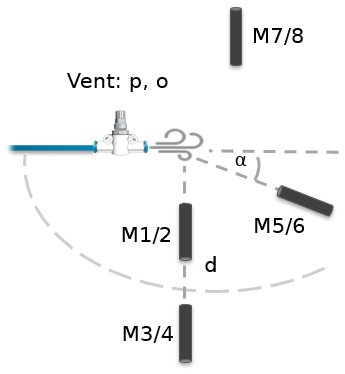
\includegraphics[width=55mm]{images/mic_positions_scheme.png}
%     \captionof{figure}{A table beside a figure}
%   \end{minipage}
%   \hfill
%   \begin{minipage}[b]{0.49\textwidth}
%     \centering
%     \begin{tabular}{ll}
%     Microphones & Position\\
%     \hline
%     \textbf{M1/2} & 20 cm distance, 90° to leakage\\
%     \textbf{M3/4}& 2 m distance, 90° to leakage\\
%     \textbf{M5/6}& 20 cm distance, $\alpha < 30°$\\
%     \textbf{M7/8}   & Ambient recording of whole room   
%     \label{tab:mics}
%     \end{tabular}
%       \captionof{table}{A table beside a figure}
%     \end{minipage}
%   \end{minipage}

% \subsection{Generating a two-class problem}

% Fig. 1 illustrates the detection process: Leakage type and internal pressure of a pipe cause turbulences (1.), which are described in radiation characteristics as well as, depending on the frequency range under consideration an acoustic profile. The space between the transmitter and receiver also has an Numerous influencing variables that influence the measurement signal. Thus the direct For example, the distance between the sound source and microphone is decisivefor signal levels and runtime-dependent effects. In addition, in practice overlaps by ambient noise and spatial influences such as reflections and diffuse sound.

% \begin{figure}[h]
% 	\centering
% 	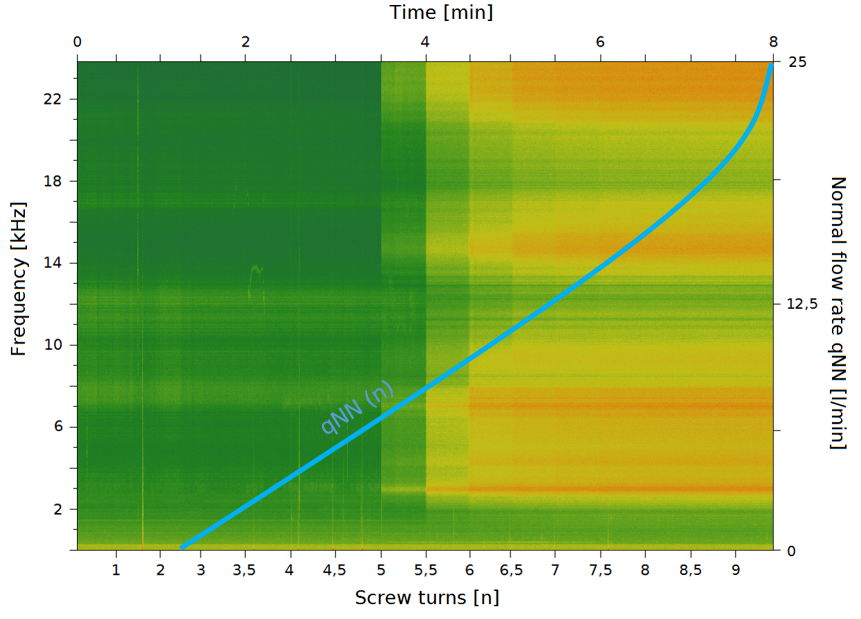
\includegraphics[width=88mm]{images/V_1_normi_qnn.png}
% 	\caption{Spectrogram of leakage noise from microfone position 1 with characteristic vent flow rate for 6 Bar}
% 	\label{fig:spec+qnn}
% \end{figure}

% The spectrogram in fig shows the recording of the leakage noise. The frequencies of the turbulently exiting air are plotted over time and the number of screw rotations. To increase visibility of the leakage sounds main features, gain is added. Recorded sound events are displayed relatively to the recording threshold level from green (low) via yellow (medium) to red (high). The knurled screw on valve two is now opened in $30s$ intervals by a fixed amount. For the interval $0 < n  3$ whole rotations are made. This action is based on consideration of the component characteristic curve (blue) from \ref{fig:spec+qnn}. From $n = 3$ half turns are made on the second screw to increase the accuracy. The resulting Recordings are later used as a reference for a leak-free environment.

% If you now look at frequencies and levels, the following becomes apparent: In the range 0 < n < 5.0 the microphone does not register any periodically occurring signal. If the screw is turned up further from $n = 5$ to $n = 5.5$ on a level maximum in the range 3.1 kHz, 7.1  kHz in the range 9.2 kHz or 14.8 kHz and beyond the audible spectrum become visible. The increasing sound level at larger n is highlighted by red coloring. For increasing screw turns the volume around those frequency bands increases the peak levels of the prominent bands however are not influenced by the screw position. Thus the average values of the frequency bands remain constant. For the upcoming measurements a signal threshold of $n = 5$ is assumed. \ref{tab:mappingclasses} links the screw turns to the two conditions \textit{no leakage/OK} and \textit{leakage/nOK}.

% \begin{table}[h]
%     \centering
% 	\begin{tabular}{ | l | c | c | c | c | c | c | c | c | c | }
% 		\hline
% 		n $=$  & 0 & . . . & 3 & 3.5 & . . . & 5 & 5.5 & . . . & 9 \\ \hline
% 		Condition & $OK$ &   . . . & $OK$ & $OK$ & . . . & $OK$ & $nOK$ & . . . & $nOK$ \\ \hline
% 		\multicolumn{1}{c}{} & \multicolumn{3}{c}{\upbracefill}& \multicolumn{3}{c}{\upbracefill}& \multicolumn{3}{c}{\upbracefill}\\[-1ex]
% 		\multicolumn{1}{c}{} & \multicolumn{3}{c}{no leak} &\multicolumn{3}{c}{leak not detectable}&\multicolumn{3}{c}{leak detectable}
% 	\end{tabular}
% 	\caption{Mapping screw turns to binary classes.}
% 	\label{tab:mappingclasses}
% \end{table}

% \subsection{Measurement series}

% % \begin{table}[h]
% %     \begin{tabular}{lll}
% %     \centering
% %     Code       & Name      & Parameters/Description\\
% %     \hline
% %     \textbf{v} & Vent Leak   & 6 Bar, choke vent, quiet lab\\ 
% %     \textbf{p} & Low Pressure Vent Leak  & 5 Bar, choke vent, quiet lab\\
% %     \textbf{o} & Damaged Tubing Leak  & 6 Bar, tubing, quiet lab\\     
% %     \textbf{w} & Vent Leak with Workshop Noise  & 6 Bar, choke vent, added aperiodic workshop ambient sounds\\
% %     \textbf{h} & Vent Leak with Hydraulic Noise & 6 Bar, choke vent, added periodic sound of screeching piston\\
% %     \textbf{ow} & Tubing Leak with Workshop Noise & \\
% %     \textbf{oh} & Tubing Leak with Hydraulic Noise & \\
% %     \textbf{pw} & Low Pressure Vent Leak with Workshop Noise & \\
% %     \textbf{ph} & Low Pressure Vent Leak with Hydraulic Noise & \\
% %     \textbf{po} & Low Pressure with Tubing Leak & \\
% %     \label{series}
% %     \end{tabular}
% % \end{table}

% \begin{table}[h]
%   \centering
%   \begin{tabular}{l l l l}
%       Code & Leak & Pressure & Noise  \\ \hline
%         \textbf{v} & Vent & Normal & None \\
%         \textbf{w} & Vent & Normal & Workshop \\
%         \textbf{h} & Vent & Normal & Hydraulic \\
%         \textbf{p} & Vent & Low & None \\
%         \textbf{pw} & Vent & Low & Workshop \\
%         \textbf{ph} & Vent & low & Hydraulic \\
%         \textbf{o} & Tube & Normal & None \\
%         \textbf{ow} & Tube & Normal & Workshop \\
%         \textbf{oh} & Tube & Normal & Hydraulic \\
%         \textbf{po} & Tube & low & None \\
%   \end{tabular}
%   \label{tab:data-var}
%   \caption{Data Variations}
% \end{table}